\chapter{はじめに}
\label{introduction}

\section{研究背景}
\label{subject}

産業革命、コンピュータによる情報革命を経て、人々を取り巻くものに機械や情報処理を含まれ高度化していく中で、ヒューマンインターフェース設計が重要となった。
ここで目指された人々と機械との最適な関係とは、「より使いやすく有用に」\footnote{国際標準化機構(ISO)による「人間中心設計」の導入部\cite{hcd}より}することとされ、エルゴノミクス、人間中心設計といった方法論がそれを具現化してきた。
この「使いやすさ」を、道具の使用における行為と結果の関係から捉えると、それは原始的な道具のように直接的であり、道具そのもに対する意識がなくなっていくような「透明化」こそが、ヒューマンインターフェースにおける理想だとされてきた。

渡邊は、その理想を実現する指針として「自己帰属感」という概念を導入し、例えばマウスカーソルやスマートフォンのような「操作時の指とグラフィックの追従性が高い」インターフェースは自身の一部や延長として感じられる、「透明」なインターフェースであると説明する。

確かにこうしたインターフェースを設計していくことは、複雑で高度な道具の力を借りて人間の活動の可能性を拡げることに貢献してきた。しかし「透明」なインターフェースを目指す一方で、人々がある目的を達成できるようになるまでの「困難」と、それを克服して自分なりのやり方を創造していくような、高度な人間の能力の発揮と喜びを感じる機会については、これまで見落とされてきたのではないだろうか。

例えば、ピアノを初めて弾くとき、奏者は手の大きさによる制約を受け、最初のうちは左右別々に指を動かすだけでも困難さを経験する。しかし、試行錯誤を経て、ピアノの制約と自身の身体能力との間で折り合いをつけていくことで、ようやく楽器を通して表現ができるようになる。ミュージシャンのスキャットマン・ジョン(ジョン・ポール・ラーキン)は、「吃音症」という発話障害を抱えながらも、「自身の身体」という切っても切り離せない存在をコントロールできない中、むしろその症状を逆手に取るように「テクノスキャット」という独自の歌唱法を開拓した。こうした思い通りにいかなさ、すなわち他者性と向き合う中で、自分なりの扱い方を見出していく過程とは、創造的で喜びのある、いわゆる「人馬一体」と言われるような関係性ではないか。

こうした関係を設計するとしたら、「それはどのようなものであるか」を深く理解し、その上で「いかに設計できるのか」という問いに取り組む必要がある。

本研究では、手指の異なる形状への変換から「身体の中の他者性」を経験させる表現を通してこの問いについて探索し、修士作品《Grasp(er)》を制作した。さらに、その体験を説明するものとして\textit{grasp}という概念を定義した。
本研究の狙いは、\textit{grasp}の観点から人と道具、機械、あるいは人体の中にある他者性との関係における「困難さ」を捉えることで、これまで見落とされてきた関係性について説明し、またそうした関係性はどのようにして引き出すことができるのかを提示することである。

\section{リサーチクエスチョン}
\label{research_question}
前節では、研究背景に触れ、本研究が「人馬一体」と言われるような、相互の折り合いをつけながら生まれる親密さについて探索するものであると説明した。ここでは、探索の上での中心的な問いについて明記する。

\begin{quote}
\textbf{対象からの影響も受けつつ、相互の折り合いをつけながら生まれる一体感はどのように生まれ、そうした関係性が芽生える状況とはいかに設計できるのか。}
\end{quote}

本研究では、「手指の異なる形状への変換」を通して「身体の中の他者性」を経験させる表現を探索することからこの問いに迫った。

\section{「身体の中の他者性」に取り組む動機}
\label{prototyping_concept_making}
本研究は、\ref{research_question}節で示した問いに、手指の異なる形状への変換から「身体の中の他者性」を経験させる表現を通してその答えや詳細な説明についての探索を試みるものである。この観点から取り組むこととしたのは、もともと抱いていた\ref{subject}節のような問題意識に対して、当初はその問題意識とは無関係に進めていた「動きのスケッチツール」という目的の習作「Digitize」を展示した際の体験者の様子が、その切り口になると捉えたことがきっかけとなったためである。
この節では、そうした着想に至るまでの経緯について説明することで、手指の異なる形状への変換から「身体の中の他者性」を経験させる表現を通してこの問いへアプローチすることの動機とする。

ここで制作した「Digitize」とは、手指の動きを別の形へとマッピングさせた3つの変換表現から構成された作品である。

静止画について構想を膨らませる際、「紙とペン」を通して直接イメージをスケッチできるが、動きについてはそれに相当するほど、直感的かつ、高い表現力でスケッチができるツールが見当たらなかった。そこで、動きに関して高い表現力を有する手指の動きを使って、「動きをスケッチする」ツールを設計することを案じていた。

しかし手指は人間の身体の中でもとりわけ随意に、高い表現力で動かすことのできる器官である。もし「手ではない形」を通してでも、様々な形や動きを自由に作れるのなら、人間の身体構造による制約を超えた「動きのスケッチ」ができるのではないか。

そうして、手指の動きをトラッキングしつつ、画面上でその動きは別の形へマッピングされて動くインターフェースについて、プロトタイピングを行い、その過程をIAMAS Open House 2022にて展示した\footnote{\url{https://k1105.github.io/eee_openhouse_2022/}}。この時点では、動きを記録する機能は存在しておらず、あくまで手と、それに伴って動く手指とは異なる形の動きが確認できるだけのものであった。

\begin{figure}[H]
  \centering
  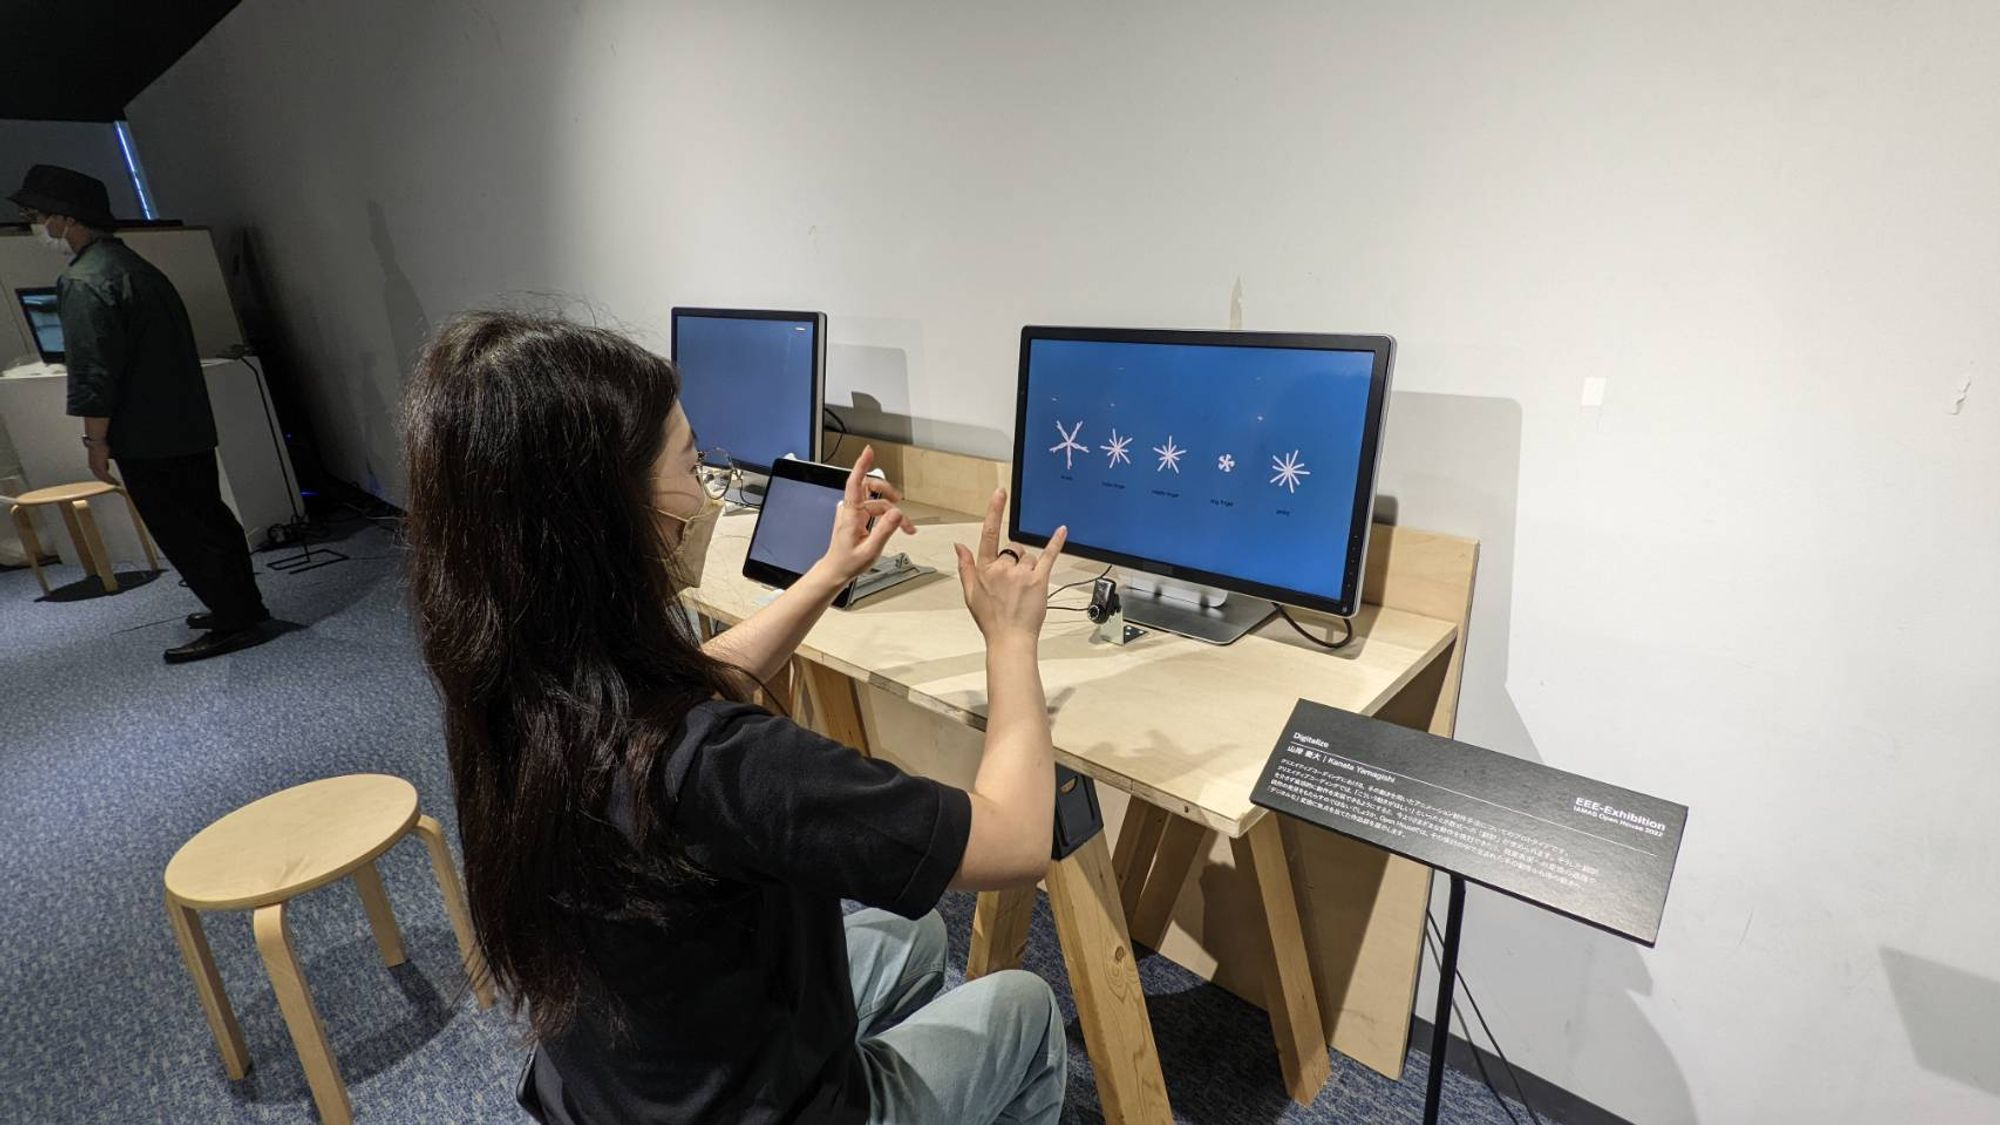
\includegraphics[width=15cm]{img/openhouse2022.jpeg}
  \caption{IAMAS Open House 2022での展示の様子(2022年)}
  \label{fig:exhibit_2022}
\end{figure}

\begin{figure}[H]
  \centering
  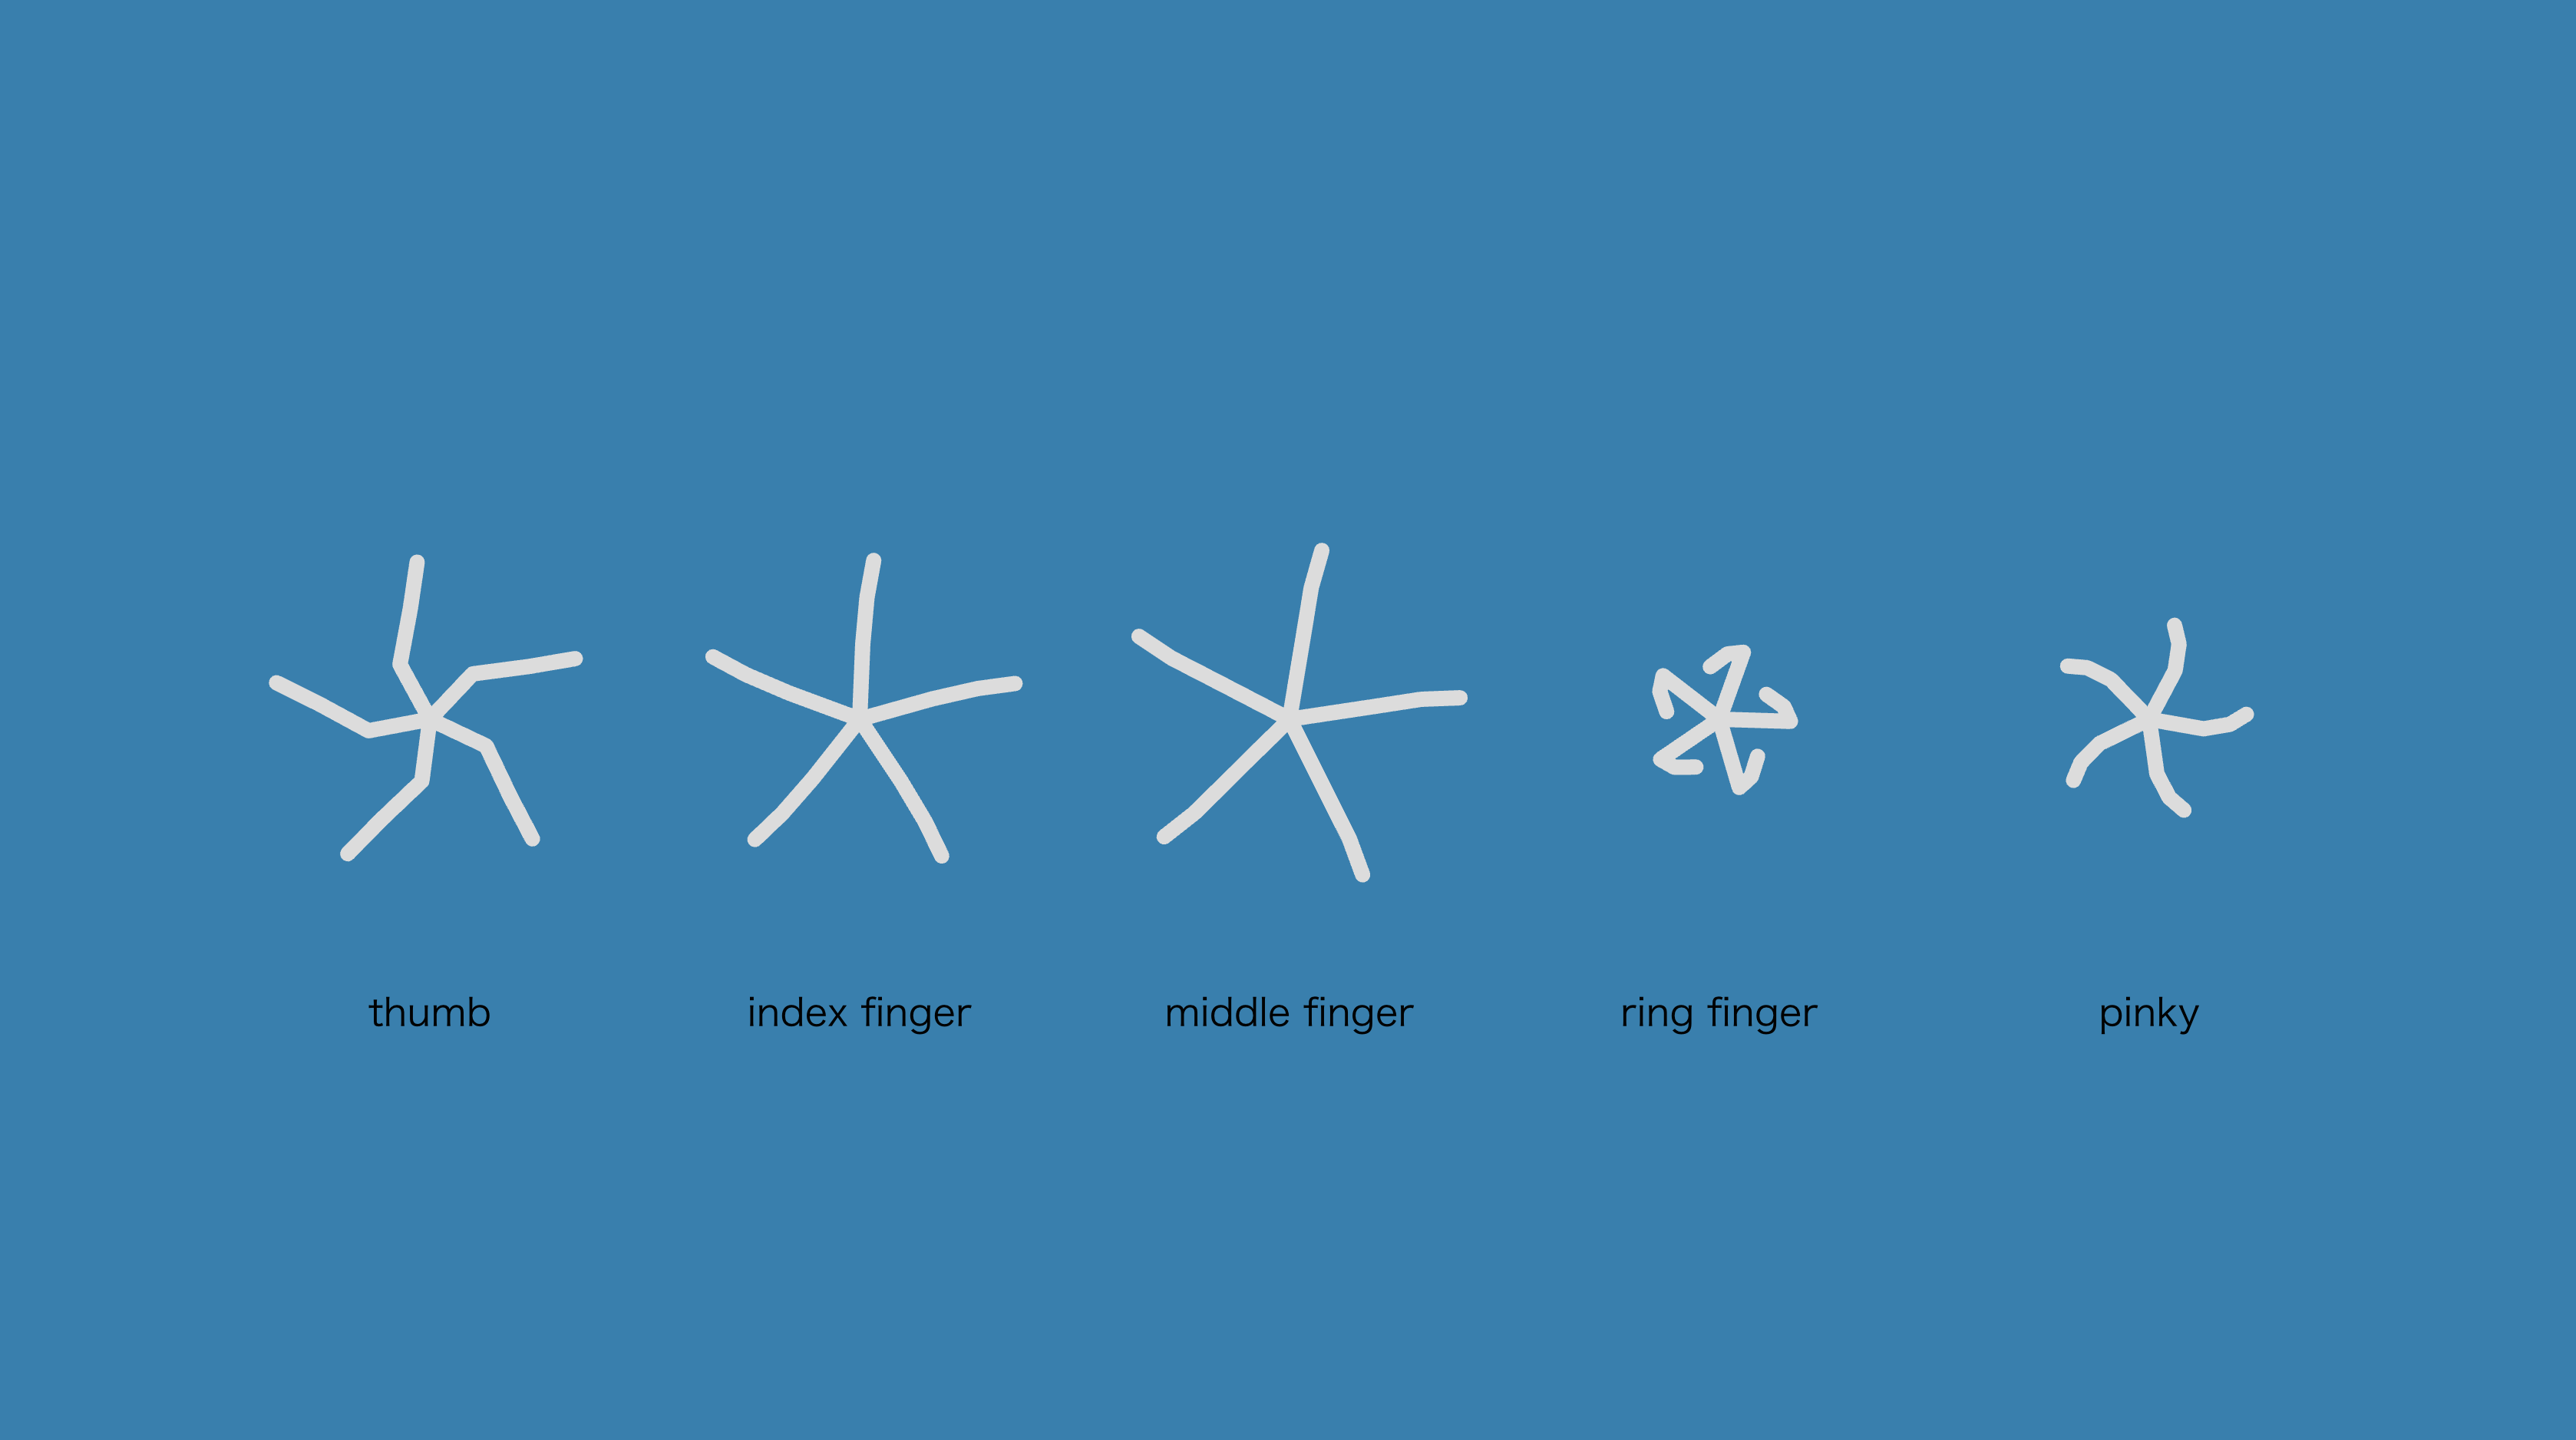
\includegraphics[width=15cm]{img/openhouse2022_interface.png}
  \caption{Digitizeのインターフェース(2022年)}
  \label{fig:exhibit_2022_interface}
\end{figure}

しかし展示を行うと、この試作には当初想定していなかった魅力があることに気づいた。それは、指の動きが単に、別の構造にマッピングされただけであるのに、別の構造の手を動かす体験はそれだけで興味を惹くものだということである。手指の異なる形状への変換が3パターン展示された状態のこの展示で、10分以上興味を持って体験する方が複数名いた。また、制作されたプロトタイプを展示した際、指先を動かすだけでなく、カメラに対して手を近づけたり遠ざけたり、手を裏返したりするなど、さまざまな体験の方法が現れた。

これは、「手指の動きに反応している」ということは分かっていても「どのように対応しているのか」がはっきりせず、それを確かめるように身体を動かしていると考えた。

仕組みを知っている制作者にとっては自明なことだが、自己の運動とどう対応するのかを知り得ない体験者は、自身の体を動かして観察されたことを通して推測することになる。それゆえに、この仕組みを通して思い描く身体像に、体験者ごとに違いがあるのではないか。

こうした体験者ごとの違いは、「わかりやすい」ものを対象としたときよりも、「わかりにくい」ものを対象としたときの方が顕著に現れると考えた。その上で、わかったようで分からない、行きつ戻りつな感覚に陥りながらも「わからなかった」と一蹴されず、それを分かろうとして向き合う様子が続いたことに、先の問題意識に応えるものがあるのではないかと考えた。


\section{研究概要}
本研究では、人間と道具や機械との関係において、人にとって道具や機械が「より使いやすく、有用に」あるという関係ではない、対象の他者性と向き合い、折り合いをつけていく経験を通して生まれる「一体感」を目指し、それがどのように生まれるのかについて探求する。この意味での「一体感」とは例えば、ピアノの演奏やバイクの運転など、人間が道具や機械の特性を理解し、使いこなすための能力を身につけることで生じる人間と対象との関係である。

この主題に、手指の異なる形状への変換を通して「身体の中の他者性」を経験させる表現を探索することから迫り、修士作品《Grasp(er)》を制作した。
また、人間と対象との関係について「Embodiment:一体化」の観点から分類したSydney Felsの4つのカテゴリや「Intimacy:親密さ」の概念に基づき、本研究では\textit{grasp}という概念を提案した。この概念を用いて本作から「一体感」が生じるまでの過程についての仮説を立て、4名の作品体験を振り返ることから、それが実現しているかについて考察する。

\section{本研究の目的}
本研究の目的は、対象の他者性と向き合い、折り合いをつけていく経験を通して生まれる「一体感」について、\textit{grasp}の観点から人と道具、機械、あるいは人体の中にある他者性との関係における「困難さ」を捉えることで、これまで見落とされてきた関係性について説明し、またそうした関係性はどのようにして引き出すことができるのかを提示することである。

\section{本論文の構成}
本章では、研究背景を問題提起の形で示し、その上でリサーチクエスチョンを提示する。また、その問いを探索する切り口として本研究が着目した「手指の異なる形状への変換」について、その観点から取り組む動機と、研究の概要を示した。

第\ref{related_works}章では、本研究の取り組みを説明するにあたり、重要な分類を行なったSydney Felsの人間と対象との関係性についての議論を紹介し、本研究の関心をより詳細に示す。その上で、これまでにどのような実践があったのか、先行事例について紹介し、本研究がどのような貢献となるのかについて示す。

第\ref{graspについて}章では、本研究が提示する\textit{grasp}について詳細に説明する。その上で、Felsの分類との関係性と、この概念を用いることから修士作品の体験についてのねらいを説明する。また、この概念に至るまでのプロトタイピングの過程を示すことで、この概念を主張する根拠とする。

第\ref{about_grasper}章では、作品概要と、そこに至るまでのプロトタイピングの分析を通して、作品形態について説明する。

第\ref{validation}章では、そのようなねらいのもと制作された本作品が、実際どのように経験されるのかについての質的調査を行うため、Video Cued Recallという手法を用いて体験について振り返り、実際の体験がどのようなものであったのかを踏まえて、モデルとの関係性について考察する。

第\ref{考察}章では、行った調査の結果からどのような体験の作品であったかを振り返り、本作品が狙いとしていたこと、あるいはその範疇を超えて、作品として何が達成されたのかについて考察する。

第7章では、これまでの議論をまとめ、最後に今後の展望として、ここで制作を行ったモデルがそれ以外の議論とどのように関係し、今後どのような可能性を有するのかについて述べる。